\section{SensorFusion}\label{section:SensorFusion}
The \textit{SensorFusion} class is implemented to adjust for yaw and pitch-rotations, where the yaw and pitch-rotation angles are provided in the constructor.
The SensorFusion adjusts the acceleration readings in the y-axis in two methods.


The method in \lstref{lst:acceleration-yaw} corrects the acceleration when the phone is tilted around the z-axis, and is important since it is affected by the gravitational pull.

When the yaw-rotation has been found, using the accelerometer and gyroscope, the gravitational pull is taken into account. 
The method, seen in \lstref{lst:acceleration-yaw}, calculates movement acceleration, without gravitational pull, is found using trigonometry.

\begin{lstlisting}[caption={Method correcting acceleration when tilted around the z-axis.}, label=lst:acceleration-yaw, float=h, style=sharpc]
private float GetAccelerationAdjustYaw(float accelerationY, float accelerationX, float gyroscopeAngle)
{
	return (float)((accelerationY - (-accelerationX * Math.Sin(gyroscopeAngle))) / (Math.Cos(gyroscopeAngle)));
}
\end{lstlisting}

An illustration of the gravitational pull problem can be seen in \figref{figure:yaw-rotation-adjustment}, which is used to explain \lstref{lst:acceleration-yaw}.

\begin{figure}[H]
	\centering
	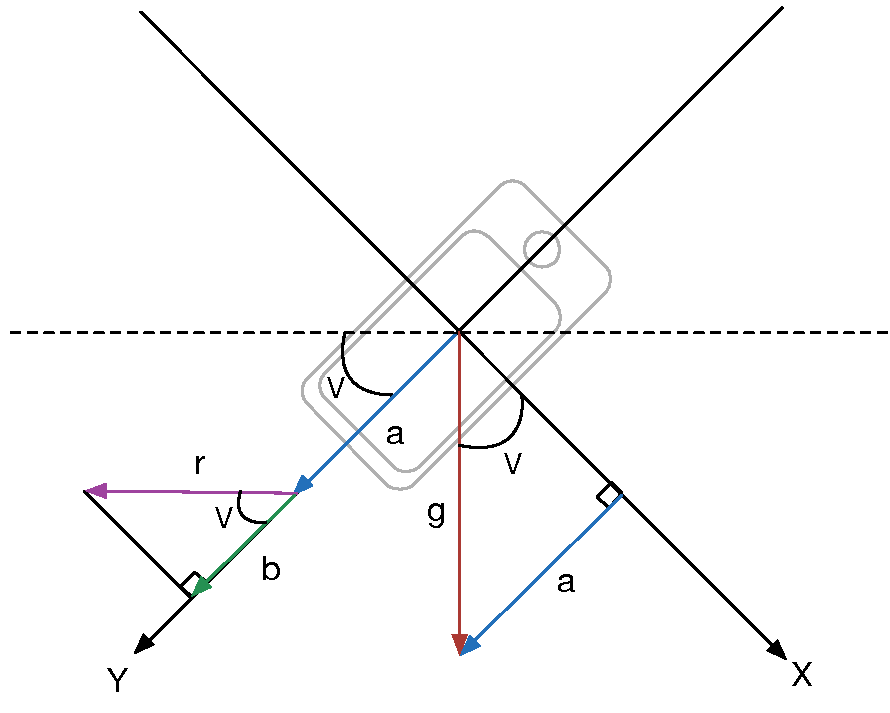
\includegraphics[trim = 0cm 0cm 0cm 3cm, clip, scale=0.75]{media/graph}
	\caption{Yaw-rotation adjustment.}
	\label{figure:yaw-rotation-adjustment}
\end{figure}

In \figref{figure:yaw-rotation-adjustment}, the phone is tilted in an angle of $V$.
$r$ is the desired acceleration, as it is the acceleration, in the y-axis, without gravitational pull. 
$a + b$, is the measured acceleration in the y-axis of the accelerometer.
$g$ is the gravitational pull, which is constant.
$g$ is used in combination with the angle $V$ to calculate $a$, which is how much the gravitational pull affects the measured acceleration in the y-axis.

\begin{equation}\label{equation:vector-a}\centering
a = g \cdot sin(V)
\end{equation}

Once $a$ has been found, using \eqref{equation:vector-a}, $b$ can be found by subtracting $a$ from the measured acceleration in the y-axis.
$b$ is the acceleration in the y-axis, unaffected by gravitational pull, however, the desired acceleration is in the horizontal plane.
As of such, $V$ and $b$, is used to find $r$, seen in \eqref{equation:vector-r}.

\begin{equation}\label{equation:vector-r}\centering
    r = \frac{b}{cos(V)}
\end{equation}

The measured acceleration in the y-axis, $m_{acc}$, is given by $a + b$.
Hence, the final formula for finding $r$ is \eqref{equation:vector-final}.

\begin{equation}\label{equation:vector-final}\centering
    r = \frac{m_{acc} - g \cdot sin(V)}{cos(V)}
\end{equation}

Much like the adjustment in the yaw-rotation, a similar correction is performed for pitch-rotation. 
However, for pitch-rotation there is no gravitational pull affecting the measured acceleration. 
For that reason, it is sufficient to use \eqref{equation:vector-r}, as $b$ is the measured acceleration.
This correction has to be calculated after the correction of the yaw-rotation.  

\begin{lstlisting}[caption={Method correcting acceleration when tilted around the x-axis.}, label=lst:acceleration-pitch, float=h, style=sharpc]
private float GetAccelerationAdjustPitch(float acceleration, float angle)
{
	return acceleration / (float)Math.Cos(angle);
}
\end{lstlisting}

The calculation of the marginal probability distribution of the SensorFusion node is not done with a direct combination.
For that reason, the variance can not be determined as the marginal distribution of the nodes that are constructed with a direct combination.
Although, the current implementation of calculating the variance of the SensorFusion node as the sum of the variance of the parents is not correct, it is done since a better solution was not present.